\chapter{Windkessel model}\label{windkessel}
This chapter introduces some concepts of physiology necessary for understanding the \textbf{Windkessel model}, later introduced. The chapter is not intended to be complete with the theory behind the model, but it is intended to introduce the idea on which it is based: the \textbf{Windkessel effect}.\\
The chapter makes use of a jupyter notebook used in the course \textit{Introduction to Python for Scientific Computing} taught by Professor Lucas Omar Müller in the academic year 2021/2022.\\
The sources used in writing the chapter are: \cite{AaronsonPhilipI.PhilipIrving2020Tcsa}, \cite{wiki:Vascularresistance}, \cite{wiki:Compliance}, \cite{wiki:WindkesselEffect},
\cite{wiki:cicloCardiaco},
\cite{wiki:DiagrammaWiggers},
\cite{westerhof_arterial_2008}, \cite{ghitti_toro_müller_2022}. \\



\begin{textblock*}{0.64\textwidth}(3.5cm+0.36\textwidth,18.5cm)
\epigraph{Medicine is a science of uncertainty and an art of probability.}{William Osler}
\end{textblock*}




\newpage

\section{Introduction}
From \cite{westerhof_arterial_2008} we consider data from a patient in whom aortic flow $Q_{text{in}}$ and systemic pressure $P$ were measured.

Viewing the graph of the two values yields what is shown in figure \ref{figDatiReali}.

\begin{figure}[h]
    \centering
    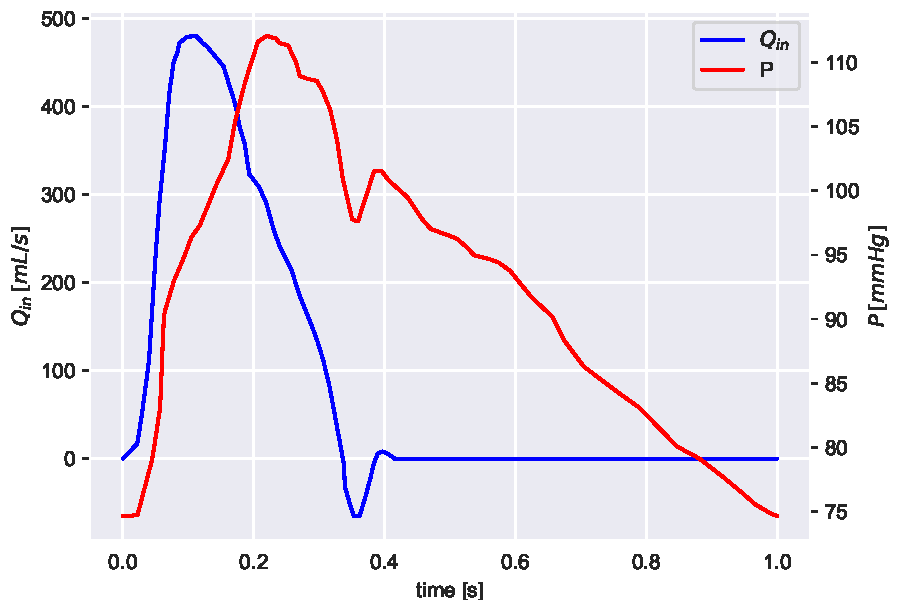
\includegraphics[width=0.7\textwidth]{images/Windkessel/DatiReali.pdf}
    \caption{Systemic pressure and aortic flow measured in a patient. Code \ref{datiReali}.}
    \label{figDatiReali}
\end{figure}

A simple model of the cardiovascular system is now considered:
\[
P=Q_{\text{in}}R,
\]
Where $R$ is the total peripheral resistance. This model allows calculation of arterial pressure from the blood flow entering the system and the total peripheral resistance.



From the patient's actual data, it is possible to derive the value of total peripheral resistance $R$, or resistance of the cardiovascular system. Given $T$ the duration of the cardiac cycle, we have:
\[
R = \frac{\frac{1}{T}\int_TP(t)dt}{\frac{1}{T}\int_TQ_{\text{in}}(t)dt}.
\]

\newpage

Having derived $R=1.037 mmHg/mL\cdot s$ (as per the code \ref{resistenzatotale}) knowing $Q_{\text{in}}$, it is now possible to use the model to derive the trend of $P$, as shown in Figure \ref{figModelloSemplic}.


\begin{figure}[h]
    \centering
    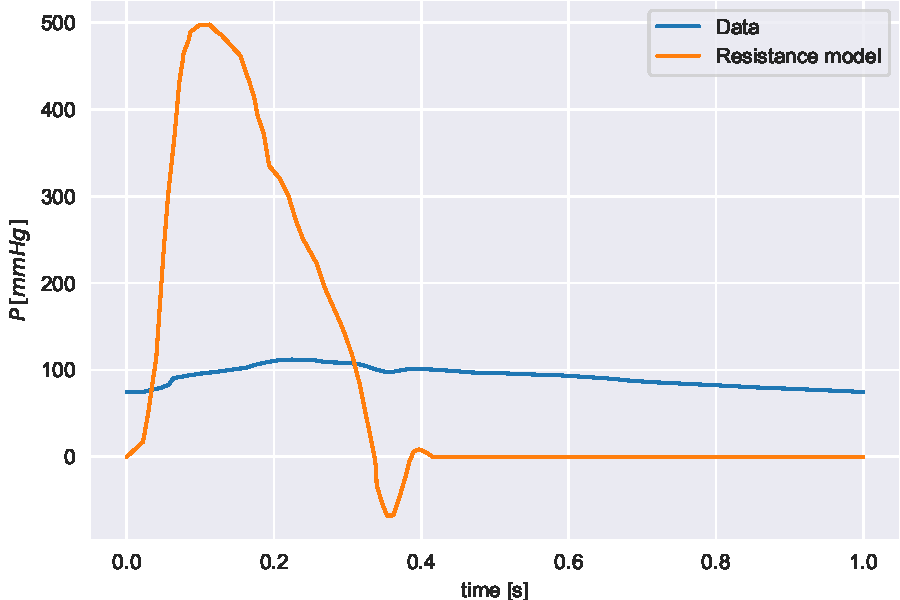
\includegraphics[width=0.7\textwidth]{images/Windkessel/modelloSemplice.pdf}
    \caption{Real pressure graph and simple model output. Code \ref{modelloSemplice}.}
    \label{figModelloSemplic}
\end{figure}

As is clear from the figure, in the systole phase the model predicts a very high peak pressure (on the order of five times higher than the actual figure). As will be shown in the rest of the chapter, this is because the model neglects a fundamental aspect of arterial circulation: the Windkessel effect, that is, the storage of energy in the arteries during the systole phase.\\
A model that takes this effect into account and thus provides a much more accurate approximation will be proposed at the end of the chapter.


\newpage




\section{Concepts of physiology}

\subsection{Cardiac cycle}
The cardiac cycle, of which a table summary is given \ref{cicloCardiaco}, will not be analyzed in detail, but the period of systole and diastole are briefly described, useful for understanding the next topics. The image \ref{wiki: cuore} may come in handy, so as to have in mind the anatomy of the human heart necessary for understanding the subsequent concepts.

\begin{figure}[h]
    \centering
    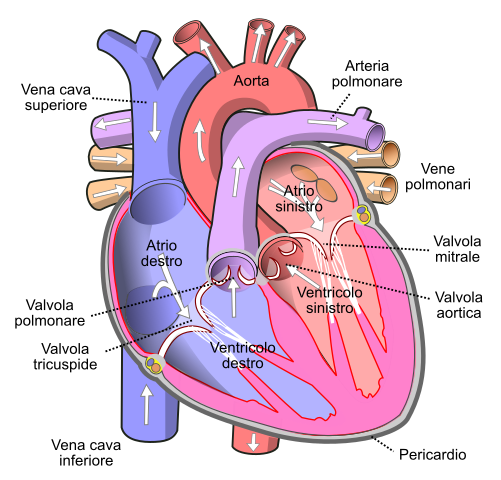
\includegraphics[width=0.7\textwidth]{images/Windkessel/Cuore.png}
    \caption{Anatomy of the human heart \cite{wiki:cicloCardiaco}.}
    \label{wiki: cuore}
\end{figure}

Cardiac diastole is the period in the cardiac cycle when, after contraction, the heart relaxes and expands as it fills with returning blood from the circulatory system. Both atrioventricular valves (tricuspid and mitral) open to facilitate the "unpressurized" flow of blood directly through the atria into both ventricles, where it is collected for the next contraction. \\

Atrial systole is the contraction of cardiac muscle cells in both atria as a result of electrical stimulation and conduction of electrical currents through the atrial chambers. \\
Defined as part of the contraction and ejection sequence, atrial systole actually plays the role of completing diastole, that is, finalizing the filling of both ventricles with blood while they are relaxed and expanded for that purpose. 

\newpage

Atrial systole overlaps with the end of diastole and applies contraction pressure to shift blood volumes to both ventricles; this atrial "kick" concludes diastole immediately before the heart begins contracting again and expelling blood from the ventricles (ventricular systole) to the aorta and arteries.\\

Ventricular systole is the contraction, following electrical stimulation, of the ventricular syncytium of heart muscle cells in the right and left ventricles. \\
Right ventricular contractions provide pulmonary circulation by pulsing oxygen-depleted blood through the pulmonary valve and then through the pulmonary arteries to the lungs. Simultaneously, left ventricular systole contractions provide systemic circulation of oxygen-depleted blood to all body systems by pumping blood through the aortic valve, aorta and all arteries.\\
Two simple diagrams depicting the displacement of oxygenated (red) and non-oxygenated (blue) blood in the systole and diastole phases are shown in Figure \ref{sistoleDiastole}.

\begin{figure}[h]
\centering
\begin{subfigure}{0.5\textwidth}
  \centering
  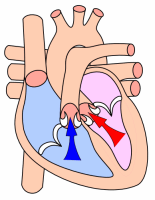
\includegraphics[width=0.5\linewidth]{images/Windkessel/sistole.png}
  \caption{Systole}
\end{subfigure}%
\begin{subfigure}{0.5\textwidth}
  \centering
  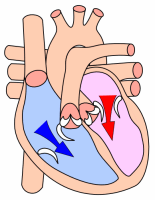
\includegraphics[width=0.5\linewidth]{images/Windkessel/diastole.png}
  \caption{Diastole}
\end{subfigure}
\caption{Diagrams summarizing the systole and diastole of a human heart \cite{wiki:cicloCardiaco}.}
\label{sistoleDiastole}
\end{figure}

\newpage

%%%%%%%%%%%%%%%%%%% TABELLA
\begin{landscape}
%%%%%%%%%%%%%%%%%%%%%%%%%%%%%%%%%%%%%%%%%%%%%%%
%%%%%%%%%%%%%%%%% TABELLA
%%%%%%%%%%%%%%%%%%%%%%%%%%%%%%%%%%%%%%%%%%%%%
% Please add the following required packages to your document preamble:
% \usepackage{graphicx}
\begin{table}
\centering
\resizebox{1.6\textwidth}{!}{%
\begin{tabular}{|l|c|c|l|}
\hline
\multicolumn{1}{|c|}{\textbf{Fase}} &
  \textbf{\begin{tabular}[c]{@{}c@{}}Valvole atrioventricolari\\ (tricuspide e mitrale)\end{tabular}} &
  \textbf{\begin{tabular}[c]{@{}c@{}}Valvole semilunari \\ (polmonare e aortica)\end{tabular}} &
  \multicolumn{1}{c|}{\textbf{Stato dei ventricoli e degli atri; flusso sanguigno}} \\ \hline
1 - Rilassamento isovolumetrico &
  chiuse &
  chiuse &
  \begin{tabular}[c]{@{}l@{}}Le valvole semilunari si chiudono alla fine della fase di eiezione; \\ il flusso di sangue si ferma.\end{tabular} \\ \hline
\begin{tabular}[c]{@{}l@{}}2a - Afflusso (riempimento \\ ventricolare)\end{tabular} &
  aperte &
  chiuse &
  \begin{tabular}[c]{@{}l@{}}I ventricoli e gli atri si rilassano e si espandono insieme; \\ il sangue scorre nel cuore durante la diastole ventricolare e atriale.\end{tabular} \\ \hline
\begin{tabular}[c]{@{}l@{}}2b - Influsso (Riempimento \\ ventricolare con sistole atriale)\end{tabular} &
  aperte &
  chiuse &
  \begin{tabular}[c]{@{}l@{}}Ventricoli rilassati ed espansi; la contrazione atriale (sistole) spinge \\ il sangue sotto pressione nei ventricoli durante la diastole ventricolare.\end{tabular} \\ \hline
3 - Contrazione isovolumetrica &
  chiuse &
  chiuse &
  \begin{tabular}[c]{@{}l@{}}Le valvole AV si chiudono alla fine della diastole ventricolare; \\ il flusso di sangue si ferma; i ventricoli cominciano a contrarsi.\end{tabular} \\ \hline
\begin{tabular}[c]{@{}l@{}}4 - Espulsione ventricolare\end{tabular} &
  chiuse &
  aperte &
  \begin{tabular}[c]{@{}l@{}}I ventricoli si contraggono (sistole ventricolare); il sangue scorre \\ dal cuore ai polmoni e al resto del corpo durante l'espulsione ventricolare.\end{tabular} \\ \hline
\end{tabular}%
}
\caption{Tabella riassuntiva ciclo cardiaco \cite{wiki:cicloCardiaco}.}
\label{cicloCardiaco}
\end{table}
%%%%%%%%%%%%%%%%%%%%%%%%%%%%%%%%%%%%%%%%%%%%%
%%%%%%%%%%%%%%% FINE TABELLA
%%%%%%%%%%%%%%%%%%%%%%%%%%%%%%%%%%%%%%%%%%
\end{landscape}

\newpage

Useful in understanding the cardiac cycle is the Wiggers diagram: this is a standard diagram that is used in teaching cardiac physiology in which the horizontal axis is used to plot time while the vertical axis contains all of the following on a single grid: blood pressure, aortic pressure, ventricular pressure, atrial pressure, ventricular volume, electrocardiogram, and arterial flow.\\
The Wiggers diagram clearly illustrates the coordinated variation of these values as the heart beats, helping to understand the entire cardiac cycle. It also helps to become familiar with the shape of the parameter curves that will be used in the paper. An example of a diagram is shown in figure \ref{WiggersDiagramma}.


\begin{figure}[h]
    \centering
    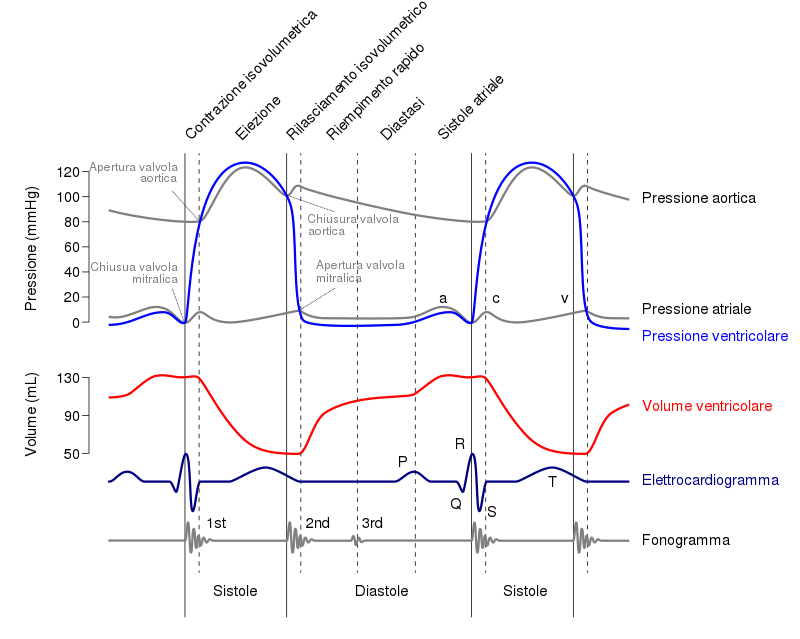
\includegraphics[width=1\textwidth]{images/Windkessel/Wiggers_Diagram_IT.svg.png}
    \caption{Example of Wiggers diagram \cite{wiki:DiagrammaWiggers}.}
    \label{WiggersDiagramma}
\end{figure}



\newpage

\subsection{Useful terminology}\label{terminologia}

%%%%%%%%%%%%  VOLUME SISTOLIC
\subsubsection{Systolic volume}
The \textbf{systolic volume} (English \textit{stroke volume}, or SV) is the amount of blood pumped from a ventricle at each ventricular systole. The systolic volume is usually equal in the two ventricles, about $70ml$ in a healthy $70kg$ man.


%%%%%%%%%%%%%%%% ELASTIC ARTERY
\subsubsection{Elastic artery}
An \textbf{elastic artery} is an artery formed by many filaments of collagen and elastin, which give it the ability to stretch in response to any pulsation. 
\\
It is by virtue of this elasticity that the Windkessel effect occurs, which helps maintain a constant pressure in the arteries despite the pulsating nature of blood flow. 
\\
Elastic arteries include the largest arteries in the body, those closest to the heart.
\\
The pulmonary arteries, the aorta and its branches together constitute the body's elastic artery system. Examples are: aorta, brachiocephalic, common carotid, subclavian, common iliac.


%%%%%%%%%%%%%%% RESISTENZA VASCOLARE
\subsubsection{Vascular resistance}
The \textbf{vascular resistance} is the resistance that must be overcome to push blood through the circulatory system and create flow. 
\\
The resistance offered by the systemic circulation is known as \textbf{systemic vascular resistance} or \textbf{total peripheral resistance} \footnote{There is the resistance offered by the pulmonary circulation known as \textbf{pulmonary vascular resistance} or PVR. However, it will not be studied in this paper}.
\\La vasocostrizione (cioè la diminuzione del diametro dei vasi sanguigni) aumenta la SVR, mentre la vasodilatazione (aumento del diametro) diminuisce la SVR.
\\
The formula is valid: $R=\frac{\Delta P}{Q}$, where $R$ is the resistance, $\Delta P$ the pressure change during the circulatory loop\footnote{That is, from just after exit from the left ventricle/right ventricle to entry into the right atrium/left atrium}, $Q$ is the flow.\\
Note that this is the hydraulic version of Ohm's law, V=IR, in which pressure differential is analogous to electrical voltage drop, flow is analogous to electric current, and vascular resistance is analogous to electrical resistance.

\newpage
%%%%%%%%%%%%% COMPLIANCE
\subsubsection{Capacity or compliance}\label{capacitanza}
The \textbf{capacity} (or compliance) is the ability of a hollow organ to stretch and increase in volume with increasing pressure. It is the fluid-dynamic equivalent of electrical capacity.\\
In the case of blood vessels, this physically means that vessels with higher compliance deform more easily than vessels with lower compliance under the same conditions of pressure and volume. \\
Venous compliance is about 30 times greater than arterial compliance, largely because of their thinner walls.\\
The $C$ compliance of a blood vessel is directly proportional to the elasticity of its walls and is a measure of the ratios of pressure changes to volume changes. It is defined as: $C=\frac{\Delta V}{\Delta P}$, where $\Delta V$ is the volume change, $\Delta P$ is the pressure change, i.e., the difference between intravascular and external pressure.\\
One feature that makes its estimation a subject of study is the difficulty of measurement: arterial compliance can be measured by several techniques, but most of them are invasive and not clinically appropriate. 

%%%%%%%%%%%%%% EFFETTO WINDKESSEL
\subsection{Windkessel effect}
The \textbf{windkessel effect} is a term used in medicine to explain the waveform of arterial pressure in terms of the interaction between the systolic volume and compliance of the aorta and large elastic arteries and the resistance of smaller arteries and arterioles.\\
Windkessel, from German, means \textit{air chamber} and was used in the 18th century by firefighters to ensure a continuous supply of water in fighting fires; in the cardiovascular case it is an elastic reservoir, but the operation is the same. Figure \ref{windkesselEffect} illustrates this analogy.

\begin{figure}[h]
    \centering
    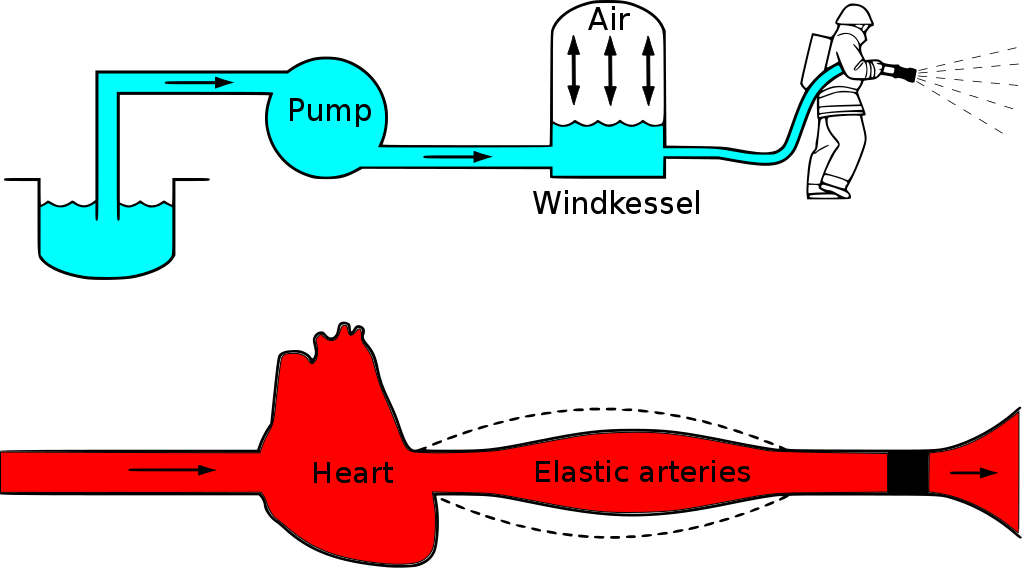
\includegraphics[width=0.7\textwidth]{images/Windkessel/WindkesselEffect.png}
    \caption{Illustration of the analogy on the windkessel effect \cite{wiki:WindkesselEffect}.}
    \label{windkesselEffect}
\end{figure}

\newpage
As introduced earlier, elastic arteries relax when blood pressure rises during systole and retract when blood pressure falls during diastole, as shown in figure \ref{windkesselEffect(libro)}. \\
Because the rate of blood entering this type of artery exceeds the rate of blood leaving, there is a net deposit of blood during systole, which is discharged during diastole. The compliance of the aorta and the great elastic arteries is thus analogous to that of a capacitor; in other words, these arteries collectively act as a hydraulic accumulator.\\
The Windkessel effect helps dampen blood pressure fluctuation during the cardiac cycle and helps maintain organ perfusion during diastole, when cardiac ejection ceases. 


\begin{figure}[h]
    \centering
    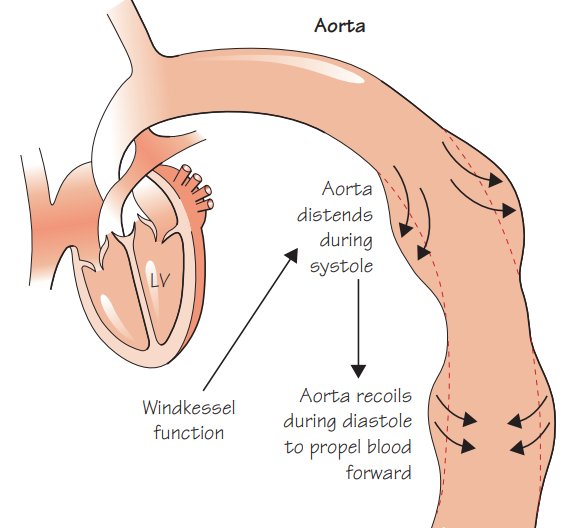
\includegraphics[width=0.7\textwidth]{images/Windkessel/WindkesselEffect(libro).PNG}
    \caption{Illustration of the windkessel effect  \cite{AaronsonPhilipI.PhilipIrving2020Tcsa}.}
    \label{windkesselEffect(libro)}
\end{figure}

\newpage

\section{Two-element Windkessel model}
Over the centuries, the arterial system has been modeled in many ways and with different strategies. An example was shown in the introduction to this chapter.
Stephen Hales\footnote{Stephen Hales (1677-1761) was an English clergyman who made important contributions to a number of scientific fields including botany, pneumatic chemistry, and physiology.} He was the first to measure blood pressure and
noted that pressure in the arterial system is not constant,
but varies over the course of the heartbeat, suggesting that
pressure variations could be related to the elasticity of the large arteries. \\
It was Otto Frank\footnote{Otto Frank (1865 - 1944) was a German physician and physiologist who contributed to cardiac physiology and cardiology} who quantitatively formulated and popularized the so-called \textbf{two-element Windkessel model}
consisting of a resistance element and a compliance element.


Poiseuille's law states that resistance is inversely proportional to the radius of the blood vessel to the fourth power. The
resistance to flow in the arterial system is therefore mainly
in the resistance vessels: the smaller arteries and the
arterioles. When all the individual resistances in the microcirculation are correctly summed, the resistance of the entire
systemic vascular bed called 
peripheral (total) resistance. The peripheral resistance, R, can
be calculated as:

\begin{equation}\label{R}
R = \frac{ P_{\text{ao; mean}}-P_{\text{ven; mean}}}{CO}\approx \frac{ P_{\text{ao; mean}}}{CO},
\end{equation}

where $P_{\text{ao; mean}}$ is the mean aortic pressure, while $P_{\text{ven; mean}}$ is the mean venous pressure, $CO$ is the cardiac output.\\
The compliance component is mainly
determined by the elasticity of the large
arteries. It can be obtained by summing the compliance
of all vessels and is therefore called total arterial compliance.\\
For the calculation of $C$ (as shown in \ref{capacitanza}), it is very difficult to perform an experiment in which a volume is injected into the arterial system without any loss in the periphery. For this reason, several methods have been developed to derive total arterial compliance without resorting to experiments.\\
The two-element Windkessel predicts that in diastole,
when the aortic valve is closed, the pressure decays
exponentially with a characteristic decay time, with which peripheral resistance can be calculated with aortic pressure in diastole and an estimate of total arterial compliance.\\
The average flow, i.e., cardiac output $CO$, is then derived from (\ref{R}). \\
The Windkessel is a so-called \textit{lumped} model. In other words, this model describes the entire arterial system
in terms of a pressure-flow relationship at its inlet,
exploiting two parameters that have physiological significance.\\
Interestingly, research in the past has mainly focused on peripheral resistance, while the contribution of total arterial compliance has often been neglected. 


The two-element Windkessel model shows how the load on the heart consists of peripheral and total arterial resistance and that both play an important role.\\

With the development of the electromagnetic flowmeter and thus the measurement of aortic flow, it became clear that in systole the relationship between pressure and flow was poorly predicted by the two-element Windkessel model. Measurements of aortic flow and developments in technological possibilities led to improvements in the two-element model: the three-element model also takes into account aortic valve resistance, while the four-element model also takes into account blood flow inertia.\\

\vspace{1cm}
To show the accuracy that the two-element Windkessel model can guarantee, the procedure in Python to obtain the pressure estimate by comparing it with the same real data used in the introductory section is shown to follow.\\
For the Python code shown, you need to import the right libraries shown in the code \ref{configurazione1}; you also need the code \ref{flusso} that defines the flow function\footnote{The code uses the real data taken from \cite{westerhof_arterial_2008}, so you need the code $\ref{datiReali}$.}.


\newpage

\subsection{Definition of the model}
As clarified in the definitions in \ref{terminologia}, the Windkessel model can be expressed in circuit form as in figure \ref{circuito}.

\vspace{1cm}

\begin{figure}[h]
    \centering
    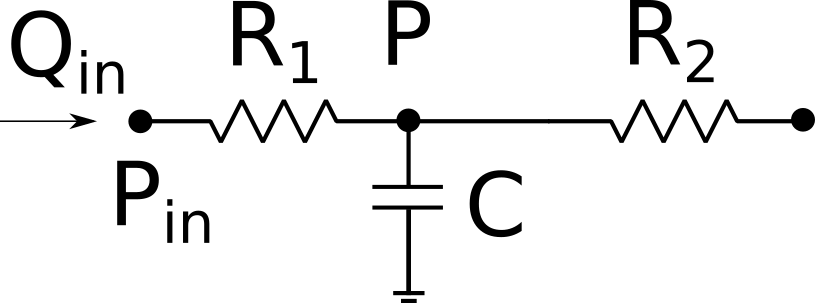
\includegraphics[width=0.6\textwidth]{images/Windkessel/Windkessel2Element.png}
    \caption{Circuit form of the two-element Windkessel model.}
    \label{circuito}
\end{figure}

The two-element Windkessel model is characterized by the equation:
\[
\frac{dP}{dt}=\frac{1}{C}(Q_{in}-Q_{out}),
\]
where $C$ is the systemic compliance, $R_1$ and $R_2$ are the proximal and peripheral resistance (of all arteries and arterioles), $Q_{out}$ the outflow from the capacitator.\\
Let us also consider $Q_{out}=\frac{P-P_d}{R_2}$, where $P_d$ is the distal pressure (i.e., subsequent to the peripheral resistance, in the course of the elaboration, when not otherwise specified, is set to $5 mmHg$), and
\begin{equation}\label{Pin}
    P_{in}=P+R_1Q_{in},
\end{equation}
from which we can then write:
\begin{equation}\label{equation}
\frac{dP}{dt}=\frac{1}{C}\left( Q_{in}-\frac{P-P_d}{R_2}\right).
\end{equation}



\subsection{Compliance estimation}
To work with the model equation, it is necessary to know compliance. To do this, you minimize the function
\[
f_C(C)=\sum_{n=1}^M\left( P_{in}(t_n)-\hat{P}_{in}(t_n)\right)^2,
\]
where $\hat{P}_{in}$ is the measured value of pressure at $M$ points $t_n$ and $P_{in}$ is defined as in (\ref{Pin}) and requires solving (\ref{equation}) with initial condition $P(0)=\hat{P}_{in}(t_1)$.\\
For this first approach it is assumed $R_1=0$ and $R_2=R$ where $R$ is the total peripheral resistance. From (\ref{Pin}) it is derived that $P_{in}=P$.\\

\newpage

Since it is necessary to solve the equation (\ref{equation}), it is necessary to define it in Python as a function, as in the code \ref{ODE}. You then define the function $f_C$ in the code \ref{fC}. The graph of the function $f_C$ is shown in figure \ref{plotfC}.

\begin{figure}[h]
    \centering
    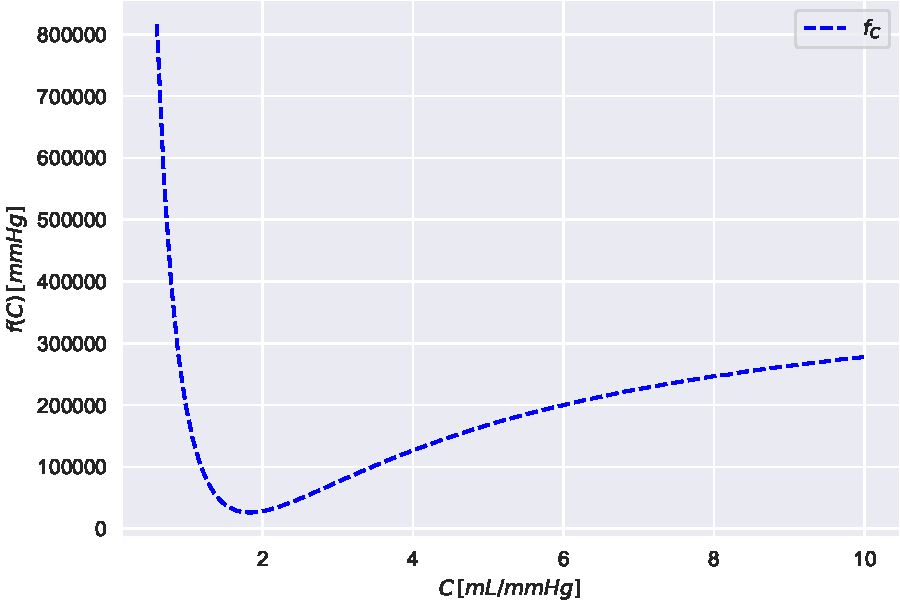
\includegraphics[width=0.75\textwidth]{images/Windkessel/f_C.pdf}
    \caption{Graph of $f_C$. Code \ref{plotfC-code}.}
    \label{plotfC}
\end{figure}



So it is now possible to estimate $C$ that minimizes $f_C$ by relying on the Python library \texttt{scipy.optimize}, as done in the code \ref{stimaC}, in this way $C=1.83288 mL/mmHg$ is found.



Now solving the equation (\ref{equation}) with the estimated $C$ yields what is in the figure \ref{soluzioneCapprossimata}.

\begin{figure}[h]
    \centering
    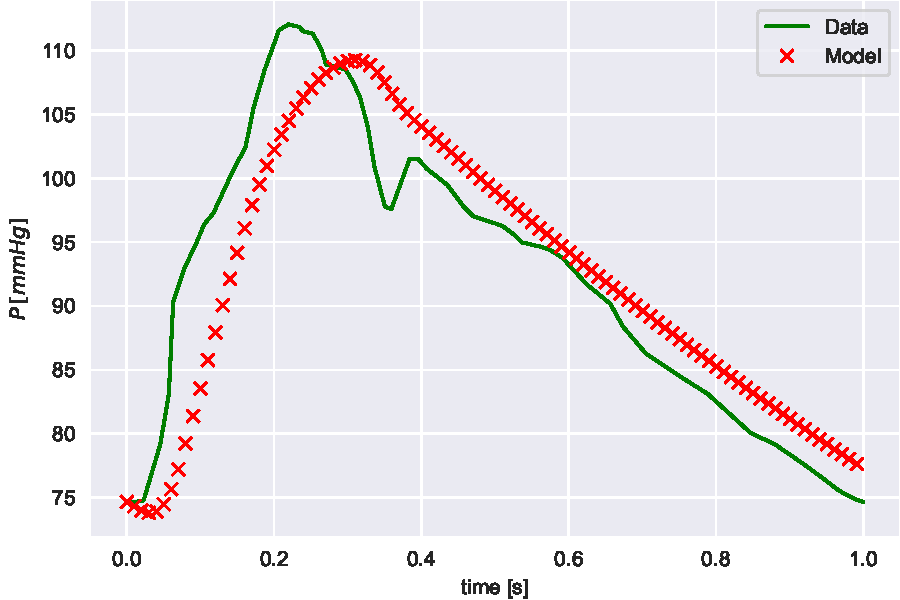
\includegraphics[width=0.75\textwidth]{images/Windkessel/modelloCstimata.pdf}
    \caption{Graph of the approximate solution of the equation (\ref{equation}) with $C$ estimated. Code \ref{plotSoluzioneCstimata}.}
    \label{soluzioneCapprossimata}
\end{figure}


\subsection{Estimation of compliance and resistance}\label{stimaCR}
By changing the definition of the resistances, the approximation can be improved. We now define: $R_1=(1-\alpha)R$ and $R_2=\alpha R$ where $\alpha\in[0,1]$. So now the function $f_C$ also depends on $\alpha$, and it is therefore necessary to update it as shown in the code \ref{fCa}.
In the code \ref{stimaCA} the parameters $C$ and $\alpha$ are estimated. We obtain: $C=2.11579 mL/mmHg$ and $\alpha=0.97134$.
Now solving the equation (\ref{equation}) with the estimated parameters of $C$ and $\alpha$ yields a graph that approximates the actual data with remarkable accuracy, as shown in figure \ref{soluzioneCalphaapprossimata}.

\begin{figure}[h]
    \centering
    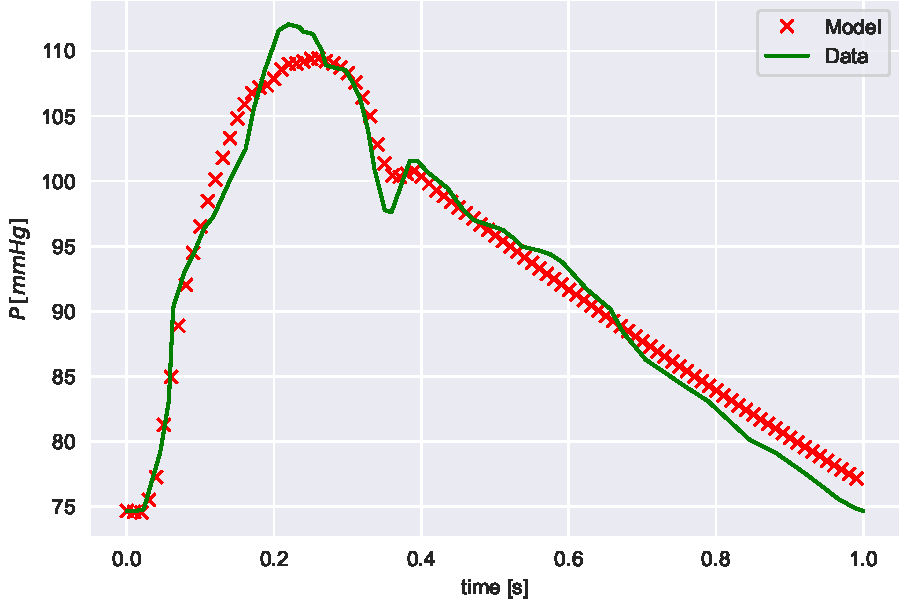
\includegraphics[width=0.75\textwidth]{images/Windkessel/modelloCalphastimata.pdf}
    \caption{Graph of the approximate solution of the equation (\ref{equation}) with $C=2,11579mL/mmHg$ and $\alpha=0,97134$. Code \ref{soluzioneCalphastimate}.}
    \label{soluzioneCalphaapprossimata}
\end{figure}


\section{Periodic forcing}
It is a well-known result that given a homogeneous linear system with constant coefficients, i.e.
\begin{equation}\label{sistema omogeneo}
    \bm{\dot{x}}(t)=A\bm{x}(t),
\end{equation}
the stability of the exact solution of that system is determined by the real part of the eigenvalues of the matrix of coefficients $A$. In particular, a necessary and sufficient condition for the system to be asymptotically stable is that all eigenvalues of $A$ have strictly negative real part. In that case there exist positive constants $\alpha, \beta$ such that
\begin{equation}\label{inequation}
||e^{At}||\leq \beta e^{-\alpha t}\quad t\geq 0.    
\end{equation}
It is now shown that when a periodic forcing function $\bm{b}(t)$ is added to the system (\ref{sistema omogeneo}) to obtain the
inhomogeneous system 
\begin{equation}\label{sistema disomogeneo}
    \bm{\dot{x}}(t)=A\bm{x}(t)+\bm{b}(t),
\end{equation}
if the homogeneous part is asymptotically stable, then any solution of the inhomogeneous system (\ref{sistema disomogeneo}) converges to a periodic solution as $t$ increases. The exact solution of the inhomogeneous system, obtained by the method of variation of constants (or Lagrange's method), is:
\[
\bm{x}(t)=e^{At}\bm{x}_0+e^{At}\int_0^t e^{A(t-s)}\bm{b}(s)ds
\]
Where $\bm{x}(0)= \bm{x}_0$. Given $\bm{b}(t)$ periodic forcing function, i.e., $\bm{b}(T_0) = \bm{b}(0)$ for some $T_0 > 0$, it is possible to obtain a periodic solution of the inhomogeneous system (\ref{sistema disomogeneo}), thus satisfying $\bm{x}(T_0) = \bm{x}(0)$, by appropriately choosing the initial condition $\bm{x}_0$. With simple math we obtain that the above initial condition $\bm{x}^P_0$ to obtain a periodic solution is given by
\[
\bm{x}_0^P=(I-e^{AT_0})^{-1} e^{AT_0}\int_0^{T_0} e^{-As}\bm{b}(s)ds.
\]
It is now shown that, starting from an initial condition other than $\bm{x}^P_0$, the solution values converge to the values of the periodic solution as $t$ increases. Let $\bm{x}^P$ be the periodic solution corresponding to the initial condition $\bm{x}^P_0$, let $\bm{x}^{NP}$ be any solution of the inhomogeneous system associated with some initial condition $\bm{x}_0^{NP}$. Then, calculating the norm of the difference between the two solutions and applying (\ref{inequation}), we obtain
\[
||\bm{x}^P(t)-\bm{x}^{NP}(t)||=||e^{At}(\bm{x}_0^P-\bm{x}_0^{NP})||\leq \beta e^{-\alpha t} ||\bm{x}_0^P-\bm{x}_0^{NP}||,
\]
in which $\beta e^{-\alpha t}\rightarrow 0$ for $t\rightarrow +\infty$, that is what was intended to be proved. 

Then if the forcing function $\bm{b}(t)$ is periodic and if the homogeneous part of the system is asymptotically stable, then the exact solution of the inhomogeneous problem will converge to the periodic solution of the inhomogeneous system itself as $t$ increases for any permissible choice of the initial condition.

\subsection{Application to the Windkessel model}
In the Windkessel model, the periodic forcing is the cardiac flux, as observed in equation (\ref{equation}). So, following the above, instead of finding an approximation of the solution using the flow of a single cardiac cycle, an approximation is found over several cycles until the solution is, barring a tolerance, equal to the previous one.

To do this, simply replace the flow function code \ref{flusso} with \ref{flusso periodico} and when solving the differential equation replace \verb|t_span| and of \verb|t_eval| with \verb|t_span = [time[0], numCycles+time[-1]]| and \verb|t_eval = numCycles+time| where \verb|numCycles| is the number of cardiac cycles against which to solve the differential equation. 

\newpage

With these changes to the code we repeat what we saw earlier for the approximation of $\alpha$ and $C$ and find: $C=2.03424$ and $\alpha= 0.97354$. The approximation of the solution after twenty cardiac cycles with these parameters is shown in figure \ref{soluzionePeriodicaCalphaapprossimata}.


\begin{figure}[h]
    \centering
    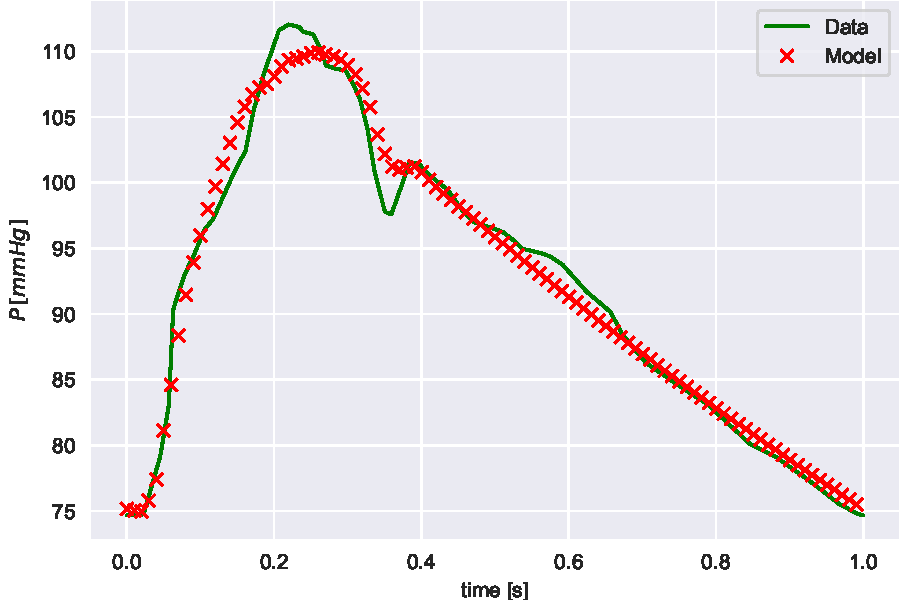
\includegraphics[width=0.75\textwidth]{images/Windkessel/modelloPeriodicoCalphastimata.pdf}
    \caption{Graph of the solution of the equation (\ref{equation}) approximated after twenty cardiac cycles with $C=2,03424mL/mmHg$ e $\alpha=0,97354$.}
    \label{soluzionePeriodicaCalphaapprossimata}
\end{figure}

Note that in the figure \ref{soluzioneCalphaapprossimata} the error of the solution approximated by the real pressure is in norm infinite $5.005246$ and in norm two $55.584739$, while in the figure \ref{soluzionePeriodicaCalphaapprossimata} in norm infinite is $4.654959$ and in norm two is $46.429220$. So the second approach, the one that takes into account the convergence of each solution to the periodic solution, generates more accurate results at the expense of more heart cycles to consider.


\subsection{Running time} \label{Windkessel: tempo esecuzione}
With the python command \verb+%%timeit -r 20+ (referred to as a \textit{built-in magic command} of jupyter notebooks) it is possible to compute the average time and standard deviation of 20 executions of python code contained in a jupyter notebook cell. When the approximation of the solution to convergence is sought, it is verified to be quite similar to the previous one, unless $5\times 10^{-3}$. As explained in \ref{Risultati training: dataset}, the input dataset consists of 3375 combinations of parameters $C, R_1, R_2$, for each of which the solution to convergence is sought. Over all the combinations we obtain different numbers of cycles required to reach convergence, all strictly less than one hundred. 

\newpage

To give an idea of how long this approach takes, shown in table \ref{tab: tempo windkessel} are the amount of time it takes to find the solution after several cardiac cycles.

\vspace{1cm}

% Please add the following required packages to your document preamble:
% \usepackage{lscape}

\begin{table}[!htb]
\centering
\begin{tabular}{cc}
\hline
\textbf{Cardiac cycles} & \textbf{\begin{tabular}[c]{@{}c@{}}Running time \\ (mean + dev. std.)\end{tabular}} \\ \hline
1   & 17.1 ms + 1.23 ms \\
10  & 90.4 ms ± 3.75 ms \\
20  & 189 ms ± 10.3 ms  \\
30  & 270 ms ± 12.9 ms  \\
40  & 362 ms ± 13.3 ms  \\
50  & 458 ms ± 15.1 ms  \\
60  & 526 ms ± 21.7 ms  \\
70  & 602 ms ± 15.9 ms  \\
80  & 711 ms ± 17.3 ms  \\
90  & 802 ms ± 32.3 ms  \\
100 & 883 ms ± 17.6 ms  \\ \hline
\end{tabular}
\caption{Run time to find the approximation of the solution of the Windkessel model over several cardiac cycles. }
\label{tab: tempo windkessel}
\end{table}





%%%%%%%%%%%%%%%%%%%%%%%%%%%%%%%%%%
%%%%%%%%% ANALISI SENSITIVITA'
%%%%%%%%%%%%%%%%%%%%%%%%%%%%%%%%
\section{Local sensitivity analysis}\label{sensitività}
In this section, the sensitivity of the model output to parameter changes is investigated by performing a \textit{local sensitivity analysis}. \\
The output of the model (the pressure $P$) is used to calculate four variables:
\begin{itemize}
  \item $\text{MAP}$: Mean Arterial Pressure, is calculated as $\text{mean}(P)$;
  \item $\text{DBP}$: Diastolic Blood Pressure, is calculated as $\text{min}(P)$;
  \item $\text{SBP}$: Systolic Blood Pressure,  is calculated as $\text{max}(P)$;
  \item $\text{PP}$: Pulse Pressure, is calculated as $\text{max}(P)-\text{min}(P)$.
\end{itemize}

\newpage

From the output obtained with the values of $C$ and $\alpha$ estimated in the code \ref{stimaCA}, the values of the variables are reported by comparing them with the actual values (of healthy individuals) in the table \ref{tab:variabili}.

% Please add the following required packages to your document preamble:
% \usepackage{graphicx}
\begin{table}[!htb]
\centering
\resizebox{0.7\textwidth}{!}{%
\begin{tabular}{cccc}
\hline
\textbf{Variables} & \textbf{Unit of measurement} & \textbf{Model} & \textbf{Real} \\ \hline
MAP                & mmHg                  & 92.91            & 65 - 110       \\
DBP                & mmHg                  & 74.86            & \textless 80   \\
SBP                & mmHg                  & 109.78           & \textless 120  \\
PP                 & mmHg                  & 34.91            & $\sim$ 40       \\ \hline
\end{tabular}%
}
\caption{Variable values calculated with the Windkessel model and input parameters ($C, \alpha$) estimated. Actual values are taken from \cite{AaronsonPhilipI.PhilipIrving2020Tcsa}.}
\label{tab:variabili}
\end{table}

The concept of local sensitivity is formalized as.
\[
S_\mathcal{M}^\mathcal{P}=\frac{\hat{\mathcal{P}}}{\hat{\mathcal{M}}} \frac{\partial \mathcal{M}(\mathcal{P})}{\partial \mathcal{P}},
\]
where $S_\mathcal{M}^\mathcal{P}$ is the sensitivity of the variable $\mathcal{M}$ to the change of the parameter $\mathcal{P}$. The values $\hat{\mathcal{M}}$ is the value calculated from the model output while $\hat{\mathcal{P}}$ is the set value of the parameter.\\

To calculate the partial derivative, use was made of the \textit{centered finite difference method} readjusted to the calculation of local sensitivity, as shown in the code \ref{differenzefinite}. Ten percent of its value was used as the variance for each parameter.

For each parameter $\mathcal{P}=\{C,R_1,R_2,P_d\}$ we then solve the problem at initial values (\ref{equation}) twice: once with the parameter increased by ten percent, once with the parameter decreased by ten percent; the other parameters are left unchanged. The two $P$ outputs obtained (along with the parameter change) are then used in the centered finite difference method for approximating the partial derivative. Finally, the sensitivity is calculated. \\
The example in the case $\mathcal{P}=C$ is shown in the code \ref{Csensitivity}.
Table \ref{tab:local sensitivity} summarizes the sensitivity values obtained in descending order in modulus.

\input{Tabelle/tabella sensitività locale}

Table \ref{tab:VariazioneParametri-Variabili} shows the variation of variables as a function of parameter variation.

\newpage

% Please add the following required packages to your document preamble:
% \usepackage{multirow}
% \usepackage{lscape}
\begin{landscape}
\begin{table}
\centering
\begin{tabular}{ccccccccccccc}
\hline
\textbf{Variables} &
  \textbf{$\text{MAP}_S$} &
  \textbf{$\text{MAP}_{+10\%}$} &
  \textbf{$\Delta_{MAP}$} &
  \textbf{$\text{DBP}_S$} &
  \multicolumn{1}{l}{\textbf{$\text{DBP}_{+10\%}$}} &
  \multicolumn{1}{l}{\textbf{$\Delta_{DBP}$}} &
  \multicolumn{1}{l}{\textbf{$\text{SBP}_S$}} &
  \multicolumn{1}{l}{\textbf{$\text{SBP}_{+10\%}$}} &
  \textbf{$\Delta_{SBP}$} &
  \textbf{$\text{PP}_S$} &
  \textbf{$\text{PP}_{+10\%}$} &
  \textbf{$\Delta_{PP}$} \\ \hline
\textbf{$C$} &
  \multirow{4}{*}{92.91} &
  91.81 &
  -1.18\% &
  \multirow{4}{*}{74.86} &
  74.92 &
  +0.08\% &
  \multirow{4}{*}{109.78} &
  107.32 &
  -2.24\% &
  \multirow{4}{*}{34.91} &
  32.40 &
  -7.19\% \\
\textbf{$R_1$} &
   &
  93.18 &
  +0.29\% &
   &
  74.91 &
  +0.07\% &
   &
  110.43 &
  +0.59\% &
   &
  35.52 &
  +1.75\% \\
\textbf{$R_2$} &
   &
  94.54 &
  +1.75\% &
   &
  74.93 &
  +0.09\% &
   &
  110.66 &
  +0.80\% &
   &
  35.73 &
  +2.35\% \\
\textbf{$P_d$} &
   &
  93.01 &
  +0.10\% &
   &
  74.86 &
  +0.00\% &
   &
  109.84 &
  +0.05\% &
   &
  34.98 &
  +0.20\% \\ \hline
\end{tabular}
\caption{Variation of variables as parameters increase by ten percent. $\mathcal{M}_S=\{\text{MAP}_S, \text{DBP}_S, \text{SBP}_S, \text{PP}_S\}$ are the variables obtained with standard (previously estimated) parameters, $\mathcal{M}_{+10\%}=\{\text{MAP}_{+10\%}, \text{DBP}_{+10\%}, \text{SBP}_{+10\%}, \text{PP}_{+10\%}\}$ are the variables obtained with individual parameters increased by ten percent, $\Delta=\{\Delta_{MAP}, \Delta_{DBP}, \Delta_{SBP}, \Delta_{PP}\}$ are the percentage changes in the subscript variable.}
\label{tab:VariazioneParametri-Variabili}
\end{table}
\end{landscape}

\newpage
From the table \ref{tab:VariazioneParametri-Variabili} it is understood that $P_d$ has low influence in all variables.\\
Local sensitivity thus behaves as expected: the higher this is (in modulus), the greater the percentage change (in modulus) in the variable by changing the parameter.\\
For example in the case $\mathcal{M}=\text{MAP}$, the change in percent is highest by modifying $R_2$, followed by the change obtained by modifying $C$, then by that by modifying $R_1$ and $P_d$. It then follows the same order as the sensitivity of $\text{MAP}$ (in modulus).\\
It can be seen that $\text{DBP}$ depends sparsely on all parameters.\\
In addition $C$ has strong influence in the variation of $\text{SBP}$ and $\text{PP}$ (the latter also influenced not insignificantly by $R_1$ and $R_2$).\\
Overall $R_2$ has greater influence than $R_1$, although the influence of the latter is not negligible.\\

Note that for each parameter the percent change in each variable has inverse sign of sensitivity. This follows from the method of centered finite differences: a negative change would result in a percent change concordant with the sign of sensitivity.